\documentclass[12pt]{article}
\usepackage{makeidx}
\makeindex
\usepackage{subcaption}
\usepackage[utf8]{inputenc}%acentuação das palavras
\usepackage[T1]{fontenc}%codificação de fonte
\usepackage[brazilian]{babel}
\usepackage{tikz}
\usepackage{textcomp}
\usepackage{afterpage}
\usepackage{varwidth}
\usepackage{indentfirst}
\usepackage{amsfonts}
\usepackage{amsmath}
\usepackage{amsthm}
%\usepackage{amssymb}
\usepackage{amscd}
\usepackage{amsxtra}
\usepackage{latexsym}
\usepackage{hyperref}
%\usepackage{cleveref}
\usepackage{enumerate}
\usepackage{fancyhdr}
\usepackage{etoolbox}
\usepackage{multicol}
\usepackage{multirow}
\usepackage{setspace} \onehalfspacing
\usepackage{mathptmx}
\usepackage[portuguese,ruled,vlined,linesnumbered]{algorithm2e}%algoritmos
\setlength{\parindent}{1.5cm}
\usepackage[a4paper,top=3cm,bottom=2cm,left=3cm,right=2cm,marginparwidth=1.75cm]{geometry}
\usepackage{lastpage}
\usepackage{fancyhdr}

\usepackage[italic]{mathastext}
\usepackage{graphicx}
\usepackage{longtable}

\title{Projeto 2 - MS960/MT862}
\author{Fernando Ribeiro de Senna --- RA 197019\\
Rodolfo da Silva Santos --- RA 228711}
\date{13 de novembro de 2020}
\begin{document}
\maketitle

Foi implementada rede neural regularizada para classificar dígitos manuscritos. Foram utilizados como exemplos de treinamento imagens provenientes da base de imagens MNIST ($20 \times 20$), linearizadas em vetores de 400 entradas. A implementação computacional foi feita em linguagem \textit{python} em três arquivos: \textit{functions.py}, que contém as funções utilizadas; \textit{neural\_networks\_p2\_1.ipynb}, que contém a parte 1 do projeto (mais voltada à implementação do algoritmo) e \textit{Avaliacao\_NeuralNet.ipynb} que contém a parte 2 do projeto (voltada à seleção de do modelo).

A Seção \ref{doc} apresenta documentação das funções implementadas no arquivo \textit{functions.py,} a Seção \ref{dados} apresenta a forma como foi feita a importação e o processamento dos dados (comum aos arquivos \textit{neural\_networks\_p2\_1.ipynb} e \textit{Avaliacao\_NeuralNet.ipynb}), a Seção \ref{parte1} versa sobre a implementação computacional da parte 1 do projeto e a Seção \ref{parte2} apresenta o que foi feito na parte 2 do projeto.

Foram utilizados funções e objetos das bibliotecas \textit{pandas, numpy} e \textit{matplotlib}. 

Toda a fundamentação teórica se baseia em conteúdo oferecido em vídeo-aulas e \textit{slides} pelo Professor João Batista Florindo em ocasião de oferecimento da disciplina MS960 no segundo semestre de 2020 pelo Instituto de Matemática, Estatística e Computação Científica (IMECC) da Universidade Estadual de Campinas (UNICAMP).


\section{Documentação} \label{doc}
Essa Seção apresenta as funções utilizadas no projeto, implementadas no arquivo \textit{functions.py.}

\subsection{Função backpropagation}
Função que realiza o treinamento da rede neural.

Argumentos de entrada:

\begin{description}
\item[X] Matriz com dados do conjunto de treinamento.

\item[y] Vetor com rótulos corretos para o conjunto de treinamento.

\item[num\_labels] (int) Número de rótulos (números) distintos no conjunto de treinamento.

\item[hidden\_layer\_size] Lista contendo o número de unidades de ativação em cada uma das camadas escondidas da rede neural.

\item[Lambda] (int) Valor de $\lambda$ a ser usado na regularização.

\item[alpha] (int) Taxa de aprendizado.

\item[nbr\_iter] (int) Número de iterações.

\item[regularizada] Booleano que indica se deve ser utilizada regularização ou não (opcional, padrão é \textit{True}).
\end{description}

A função retorna:

\begin{description}
\item[theta] Lista de \textit{arrays} contendo os valores dos parâmetros $\Theta$ obtidos pelo treinamento

\item[J\_history] Lista com os valores da função de custo para cada iteração
\end{description}

A função cria uma lista de \textit{arrays} inicializados aleatoriamente pela função \textit{randInitializeWeights} com dimensões coerentes com a arquitetura da rede neural fornecida pelo usuário. Em seguida, é realizado o treinamento utilizando a função \textit{gradientDescent}, obtendo, com isso, os argumentos de saída da função.

\subsection{Função computeCost}
A função ComputeCost calcula o custo e a saída da rede neural. Para isso está função executará o algoritmo de forward e o algoritmo de backpropagation da rede neural. Todas as informações da rede foram armazenadas em vetores, matrizes ou lista, permitindo a escolha do número de entradas na primeira camada, o número de camadas escondidas e o número de saídas na última camada, bem como o número de unidades de ativação em cada camada.

Argumentos de entrada: 
\begin{description}
\item[X] Matriz com dados do conjunto de treinamento.
\item[y] Vetor com rótulos corretos para o conjunto de treinamento
\item[theta] Lista contendo vetores de pesos de cada camada de ativação da rede neural, inicializados randomicamente pela função randInitializeWeights. 
\item[num\_labels] (int) Número de rótulos (números) distintos no conjunto de treinamento.
\item[hidden\_layer\_size] Lista contendo o número de unidades de ativação em cada uma das camadas escondidas da rede neural.
\item[input\_layer\_size] (int) Número de unidades de ativação da camada de entrada.
\item[Lambda] (int) Valor de Lambda a ser usado na regularização.
\item[regularizada] Booleano que indica se deve ser utilizada regularização ou não (opcional, padrão é True).
\end{description}

A função retorna: 

\begin{description}
\item[cost] (float) custo médio da rede ou custo regularizado.
\item[grad] Lista de vetores contendo os gradientes médios ou gradientes regularizados. 

\end{description}
A função computeCost começa inicializando o custo \textbf{J = 0}, o vetor \textbf{X} (acrescentando o bias) e a matriz \textbf{y10} que é inicializado com todos os valores zerados e com dimensão m x num\_labels, ou seja, o número de treinamentos x número de classes. Uma vez que cada exemplo de treinamento terá uma saída em \textbf{y10}. Em seguida a matriz \textbf{y10} recebe valores iguais a 1 nas entradas que batem corretamente com as entradas do vetor \textbf{y}.

No foward foi criada a lista \textbf{an} para armazenar todas as saídas das camadas de ativações como matrizes. A matriz \textbf{X} foi colocada na primeira posição de \textbf{an} para facilitar o cálculo dos demais elementos de \textbf{an}. Entre cada uma das camadas de ativação foi feito uma regressão logística \textbf{(sigmoid(an[i] @ thetan[i].T))} e o resultado armazenado em \textbf{an}. Em cada saída de camada de ativação, exceto a primeira (que armazenou o \textbf{X}) e a última (camada de saída), foram colocados os \textbf{bias}.

Por fim, a função de custo J é calculada por meio da seguinte função:

$J(\theta) = -1/m \sum^{m}_{i=1}\sum^{k}_{k=1} y^{(i)}_{k} log(h_{\theta}(x^{(i)})_{k})+(1 - y^{(i)}_{k})log(1 - (h_{\theta}(x^{(i)})_{k})) $

Por fim o custo regularizado é calculado. 

No backpropagation começamos criando uma lista \textbf{(grad)} para armazenar os gradientes de cada camada. Iniciamos a lista \textbf{grad} com matrizes no mesmo formato que as matrizes da lista \textbf{theta}, só que com todas as entradas com zero.
Em seguida é calculada a atualização dos pesos theta através da acumulação das derivadas. Assim sendo o seguinte algoritmo é executado:
Para cada entrada/imagem do vetor \textbf{X}:
\textbf{xi} – vetor com a entrada i de \textbf{X}.
\textbf{ani} – que recebe a ativação \textbf{an[i,:]} do exemplo i. Para cada entrada de \textbf{an}, exceto a primeira que contem \textbf{X}.
Em seguida calculam-se os deltas (erros da rede) fazendo-se o caminho inverso, ou seja, começa pelo o último, em seguida o penúltimo, até se chegar ao primeiro.

O erro da unidade de saída é calculado fazendo-se $\delta^{L}_i = a^{L}_{i} - y$.
Nas demais n-1 camadas aplica-se a formula $\delta^{n}_{i} = \theta^{(n)}_{1i}\delta^{(n+1)}_{1}(1-a^{(n)}_{i})$ para se calcular o erro. Sendo n a camada a qual está sendo calculado o erro e i o índice da unidade de ativação da camada. 

Em seguida calculamos o gradiente médio (derivada média) com grad[j] = 1/m*grad[j] para cada camada de ativação j. E por fim o gradiente regularizado.

Se a opção regularizada for escolhida o custo e o gradiente regularizados serão retornados no final, caso contrario a função retornara o custo e gradiente médios.


\subsection{Função gradientDescent}
Calcula o gradiente descendente atualizando os pesos das camadas da rede neural a cada interação. Utiliza para isso os valores da matriz grad retornada pela função computeCost e a taxa de aprendizagem alpha. Ao final de cada iteração o custo é armazenado no vetor J\_history.


Argumentos de entrada:
\begin{description} 

\item[X] Matriz com dados do conjunto de treinamento.
\item[y] Vetor com rótulos corretos para o conjunto de treinamento
\item[theta] Lista contendo vetores de pesos de cada camada de ativação da rede neural inicializados randomicamente.
\item[num\_labels] (int) Número de rótulos (números) distintos no conjunto de treinamento.
\item[hidden\_layer\_size] Lista contendo o número de unidades de ativação em cada uma das camadas escondidas da rede neural.
\item[input\_layer\_size] (int) Número de unidades de ativação da camada de entrada.
\item[lambda] (int) Valor de lambda a ser usado na regularização.
\item[regularizada] Booleano que indica se deve ser utilizada regularização ou não (opcional, padrão é True).
\item[alpha] (int) Taxa de aprendizado.
\item[nbr\_iter] (int) Número de iterações.
\end{description}
A função retorna: 
\begin{description}
\item[theta] Lista de vetores contendo os valores dos parâmetros obtidos pelo treinamento
\item[J\_history] Vetor com os valores da função de custo para cada iteração 
\end{description}

\subsection{Função prediction}

A função prediction faz a predição de novos exemplos após o treinamento da rede neural. Para isso ela calcula a saída da rede, ou seja, faz o forward da rede.

Atributos de entrada:

\begin{description}
\item[X] – Novos exemplos para receberem a avaliação da rede neural já treinada.
\item[theta] – Lista contendo vetores de pesos de cada camada de ativação da rede neural aproximados pela função gradientDescent.
\end{description}
A função retorna:

O  índice da maior valor da última entrada do vetor \textbf{an}.
\subsection{Função checkGradient}

Realiza a checagem do gradiente descendente da rede neural. Os detalhes do funcionamento desta função estão na seção 3.2.

Argumentos de entrada:
\begin{description} 

\item[\_X] Matriz com dados do conjunto de treinamento.
\item[\_y] Vetor com rótulos corretos para o conjunto de treinamento
\item[theta] Lista contendo vetores de pesos de cada camada de ativação da rede neural inicializados randomicamente.
\item[num\_labels] (int) Número de rótulos (números) distintos no conjunto de treinamento.
\item[hidden\_layer\_size] Lista contendo o número de unidades de ativação em cada uma das camadas escondidas da rede neural.
\item[input\_layer\_size] (int) Número de unidades de ativação da camada de entrada.
\item[lambda] (float) Valor de $\lambda$ a ser usado na regularização.
\item[regularizada] Booleano que indica se deve ser utilizada regularização ou não (opcional, padrão é True).
\item[eps] (Float) Valor de aproximação do gradiente.
\item[nbr\_iter] (int) Número de iterações.
\end{description}
A função retorna: 
\begin{description}
\item[grad] Lista de vetores com os valores do gradiente calculado pela rede neural.
\item[grad\_approx] Lista de vetores com os valores do gradiente aproximado calculado pelo algoritmo de checagem da rede neural.
\end{description}

\subsection{Função gradientConjugate}

Calcula o gradiente conjugado da rede neural regularizada. Os detalhes de implementação do gradiente conjugado estão na seção 3.3.

Argumentos de entrada:
\begin{description} 

\item[X] Matriz com dados do conjunto de treinamento.
\item[y] Vetor com rótulos corretos para o conjunto de treinamento
\item[num\_labels] (int) Número de rótulos (números) distintos no conjunto de treinamento.
\item[hidden\_layer\_size] Lista contendo o número de unidades de ativação em cada uma das camadas escondidas da rede neural.
\item[input\_layer\_size] (int) Número de unidades de ativação da camada de entrada.
\item[lambda] (int) Valor de $\lambda$ a ser usado na regularização.
\item[regularizada] Booleano que indica se deve ser utilizada regularização ou não (opcional, padrão é True).
\item[nbr\_iter] (int) Número de iterações.
\end{description}

A função retorna: 
\begin{description}
\item[res] Objeto com vários atributos. Sendo os mais importantes: vetor da solução, sinalizador booleano indicando sucesso ou fracasso e uma mensagem que descreve a causa do encerramento.
\end{description}

\subsection{Função randInitializeWeights}

Está função inicializa os pesos da rede neural de forma aleatória e de modo a benificiar a convergencia do gradiente. 

Argumentos de entrada:
\begin{description}
\item[L\_in] número de unidades de ativação na camada entrada.
\item[L\_out] número de unidades de ativação na camada de saída.
\end{description}
A função retorna:
\begin{description}
\item[w] vetor criado randomicamente com o comprimento igual à quantidade de pesos da camada mais o bias (Pesos que ficam entre as camadas \textbf{L\_in} e \textbf{L\_out})
\end{description}

\subsection{Função sigmoid}
Função de ativação da rede neural.

$1/1+e^{-z}$

Argumentos de entrada:
\begin{description}
\item[z] produto entre as saídas das camadas de ativação e seus respectivos pesos. 
\end{description}

A função retorna:
\begin{description}
\item[$1/1+e^{-z}$] função sigmoid em -z
\end{description}

\subsection{Função sigmoidGradient}
Calcula a derivada da função sigmoid

Argumentos de entrada:
\begin{description}

\item[z] produto entre as saídas das camadas de ativação e seus respectivos pesos. 
\end{description}

A função retorna:
\begin{description}
\item[sigmoid*(1-sigmoid)] derivada da função sigmoid em -z.
\end{description}

\subsection{Função reshapeTheta}
Recebe theta como um vetor e transforma em uma lista de vetores com tamanhos apropriados para cada camada de ativação da rede neural.

Argumentos de entrada:
\begin{description}
\item[theta] Vetor de pesos das camadas de ativação da rede neural inicializado randomicamente.
\item[num\_labels] (int) Número de rótulos (números) distintos no conjunto de treinamento.
\item[hidden\_layer\_size] Lista contendo o número de unidades de ativação em cada uma das camadas escondidas da rede neural.
\item[input\_layer\_size] (int) Número de unidades de ativação da camada de entrada.
\end{description}

A função retorna:
\begin{description}
\item[theta] Lista contendo vetores de pesos de cada camada de ativação da rede neural inicializados randomicamente.
\end{description}

\subsection{Função zero\_col}
Função que remove colunas (de um \textit{dataframe}) em que todas as entradas são nulas.

Argumento de entrada:

\begin{description}
\item[df] \textit{Dataframe}
\end{description}

Argumentos de saída:
\begin{description}
\item[df] Matriz contendo os dados do \textit{dataframe}, após serem removidas as colunas em que só haviam zeros.

\item[zero\_cols] Lista contendo os índices das colunas removidas.
\end{description}

A função percorre o \textit{dataframe} verificando quais colunas são nulas, as remove e armazena seus índices em uma lista. Por fim, retorna o \textit{dataframe} (convertido em matriz e sem as colunas nulas) e a lista dos índices das colunas nulas.

\section{Importação e processamento dos dados} \label{dados}
Esse processamento de dados é comum a ambas as partes do projeto e está presente nos arquivos \textit{neural\_networks\_p2\_1.ipynb} e \textit{Avaliacao\_NeuralNet.ipynb}.

Para importação dos dados, foi utilizada a função \textit{read\_csv} da biblioteca \textit{pandas}, para importar as imagens do arquivo \textit{imageMNIST.csv} e os números a que correspondem do arquivo \textit{labelMNIST.csv.} Uma vez importados os dados, foi realizada remoção de dados excessivos.

No conjunto de exemplos de treinamento, havia alguns \textit{pixels} que apresentavam valor nulo para todas as imagens presentes no conjunto de treinamento. Assim, a fim de evitar a presença excessiva de atributos na rede neural, as colunas da base de dados correspondentes a essas imagens foram removidas, já que não interfeririam no resultado. Essa transformação é feita pela função \textit{zero\_col}.

Por fim, definem-se as variáveis X e y, que são, respectivamente, uma matriz em que cada linha representa os \textit{pixels} de uma imagem do conjunto de treinamento e um vetor com os rótulos corretos do conjunto de treinamento.

\section{Implementação do Algoritmo --- Parte I} \label{parte1}
As operações descritas nessa Seção estão no arquivo \textit{neural\_networks\_p2\_1.ipynb} e são relativas à primeira parte do projeto. A importação e o processamento dos dados foram feitos conforme descrito na Seção \ref{dados}.

\subsection{Rede Neural Regularizada}

Foi implementada uma rede neural regularizada com uma camada escondida de 25 neurônios. A rede nural também permite criar testes com um número qualquer de camadas escondidas e neurônios em suas camadas de entrada, saída e escondidas. 

Os detalhes da implementação da rede neural regularizada estão demonstrados nas descrições das funções presentes na seção 2. Estas funções estão localizadas no arquivo functions.py.


\subsection{Checagem do Gradiente}

A função checkGradiente foi criada para checar o gradiente. Amostras aleatórias para a entrada \textbf{X}, a saída \textbf{y} e o theta foram criadas com tamanhos adequados e reduzidos para testar a rede em um tempo razoável.

A função checkGradiente utiliza a função computeCost para obter o gradiente aproximado para cada entrada do theta. Dessa forma, para cada entrada i de theta, calculou-se o gradiente aproximado usando a função computeCost e fazendo $\theta^{(n)}_{i}$ + $\epsilon$ (custo +) e $\theta^{(n)}_{i}$ - $\epsilon$ (custo -). Assim, a entrada correspondente aos theta[i] no gradiente aproximado vai ser calculada por $((custo+) - (custo-))/2*\epsilon$. Ao se repetir esse processo para cada entrada de theta - sempre voltando theta ao valor inicial - obteve-se o gradiente aproximado. Por causa do projeto inicial da função computeCost receber o theta já estruturado de acordo com o número de camadas da rede optou-se por não transformá-lo em um único vetor no processo.

Ao final desse processo utilizou-se, apenas uma vez, a função computeCoste para obter o gradiente gerado pela rede neural.  Por causa da forma que são armazenados, tanto o gradiente aproximado como o gradiente foram transformados em um vetores para facilitar a comparação. A comparação entre o gradiente aproximado e o gradiente foi feita por 

\begin{center}
$||grad\_approx - grad||_{2}/(||grad\_approx||_{2} + ||grad||_{2})$.
\end{center}

Essa fórmula calcula a distância euclidiana normalizada pela soma da norma dos vetores. Usou-se normalização para evitar problemas no caso de um dos vetores serem muito pequeno.. Se o valor retornado por essa formula for menor que o valor do $\epsilon$ escolhido ( $10^{-4}$) o gradiente estará correto, caso contrário o gradiente estará errado.


\subsection{Gradiente Conjugado}

No cálculo do gradiente conjugado foi utilizada a função minimize da biblioteca scipy.otimize para encontrar valores para theta de forma a minimizar a função computeCost. A função minimize recebe como argumentos de entrada uma função, um vetor com valores reais de entrada (variáveis independentes) a serem manipulados de forma que se encontre o mínimo da função de entrada, os argumentos da função de entrada e diversos outros argumentos opcionais. Por exemplo: número de interações, método de otimização e restrições. 

Dessa forma, a lista theta teve que ser convertida em um vetor para que pudesse ser manipulada pela função minimize e no processo de minimização apenas o valor do custo seria retornado pela função computeCost a função minimize.

Dentre os diversos métodos disponibilizados pela função minimize para encontrar o mínimo da função de entrada escolheu-se utilizar o método padrão BFGS (Broyden – Fletcher – Goldfarb – Shanno). Esse método pertence ao conjunto de técnicas de otimização chamadas de quase-Newton, pois ao medir a mudança no gradiente de uma interação a outra da função fornecida, ele é capaz de criar um modelo que permite convergência para valores mínimos da função. A função minimize recebeu como número máximo de interações o valores entre 200 e 1000. 

Os valores de retorno da função minimize são: Um vetor com o resultado, um valor booleano indicando sucesso ou falha no processo de otimização e uma mensagem indicando o motivo da interrupção do processo de otimização. 

\begin{center}
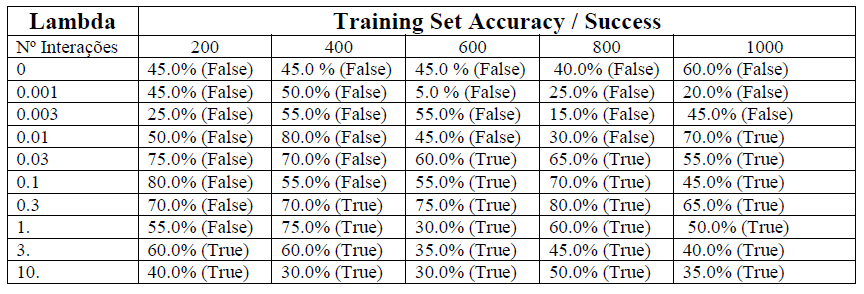
\includegraphics[width=15cm]{gradconj.PNG}

\textbf{Tabela 1 - Testes com o gradiente conjugado.}
\end{center}

Na tabela acima são apresentados diversos teste feitos com o gradiente conjugado na rede neural regularizada. A rede foi testada com 3 unidades na camada de entrada, 5 na camada escondida e 3 na camada de  saída e com 3 exemplos de treinamento.

Os testes foram feitos variando os números de interações de 200 á 100 e o valor do $\lambda$ no conjunto ${0, 0.001, 0.003, 0.01, 0.03, 0.1, 0.3, 1., 3., 10.}$. Como apresentado na tabela a tendência do gradiente conjugado convergir (Valor True) aumentou com o número de interações e com o valor de $\lambda$ . Entretanto, a taxa de precisão no conjunto de treinamento sempre apresentou melhores resultados com valores medianos de $\lambda$, ou seja, $\lambda$ muito pequenos ou muito grandes prejudicaram a taxa de acertos. 


\subsection{Visualização das unidades de ativação escondidas}
A fim de ser possível visualizar a contribuição de cada unidade de ativação escondida, foi representado gráficamente o vetor de parâmetros $\Theta^{(1)}$ (após realização do \textit{backpropagation}), que contém os parâmetros que "transportam" \ os dados de entrada para cada unidade de ativação da camada escondida.

Para isso, removeu-se o \textit{bias} de cada uma das linhas (cada linha corresponde a uma unidade de ativação) e acrescentaram-se os valores de $\Theta^{(1)}_{i,j}$ que correspondem aos \textit{pixels} que são nulos em todas as imagens e foram retirados dos exemplos de treinamento conforme discutido na Seção \ref{dados}. O valor desses parâmetros inseridos é zero, pois não contribuem com os resultados obtidos na base de dados utilizados.

Em seguida, os valores dos parâmetros foram normalizados a fim de facilitar a visualização. Para isso, utilizou-se (com relação a cada unidade de ativação) o processo de \textit{scaling}, em que cada valor é substituído pela divisão entre a diferença entre o valor e o valor mínimo e a diferença entre os valores máximo e mínimo, conforme pode ser visto na Equação \ref{scaling}.

\begin{equation} \label{scaling}
\Theta^{(1)}_{i,j} := \frac{ \Theta^{(1)}_{i,j} - \min\limits_i\left\{\Theta^{(1)}_{i,j}\right\}}{\max\limits_i\left\{\Theta^{(1)}_{i,j}\right\} - \min\limits_i\left\{\Theta^{(1)}_{i,j}\right\}}
\end{equation}

Por fim, cada linha de $\Theta^{(1)}_{i,j}$ é rearranjada em imagem de dimensão $20 \times 20$ \textit{pixels} e impressa com auxílio de funções da biblioteca \textit{matplotlib.} A Figura \ref{img_un_escond} apresenta a representação gráfica de cada uma das unidades de ativação escondidas após realizar treinamento com todas as 5 mil imagens do conjunto de treinamento através da função \textit{backpropagation} com uma camada escondida com 25 unidades de ativação, $\lambda = 0,001, \ \alpha = 0.8$ e 800 iterações.

\begin{figure}
\begin{center}
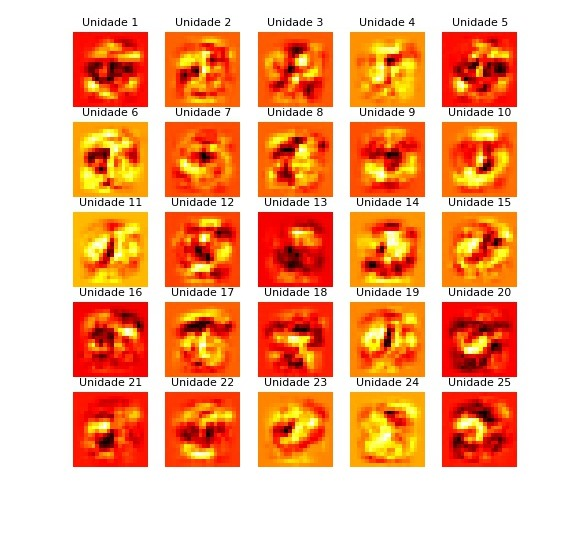
\includegraphics[scale=0.8]{corte_unidades_ativacao.jpg}
\caption{Representação gráfica das unidades de ativação da camada escondida.} \label{img_un_escond}
\end{center}
\end{figure}

\section{Seleção de modelo --- Parte II} \label{parte2}
As operações descritas nessa Seção estão no arquivo \textit{Avaliacao\_NeuralNet.ipynb} e são relativas à segunda parte do projeto. A importação e o processamento dos dados foram feitos conforme descrito na Seção \ref{dados}.


\subsection{Treino, validação e teste} \label{treino, val, teste}
\indent Inicialmente, os 5 mil exemplos de treinamento foram separados em 3 conjuntos distintos: treino, validação e teste, com 60\%, 20\% e 20\% do total de exemplos, respectivamente. Essa divisão foi feita de forma aleatória, utilizando a função \textit{random.permutation} da biblioteca \textit{numpy}.

A fim de garantir que não haveria desbalanceamento de classes, isto é, que um conjunto contivesse mais imagens correspondentes a um número do que a outro, essa separação aleatória foi feita classe a classe, de modo que no fim, 60\% dos exemplos referentes a cada número estivesse no conjunto de treino, 20\% no de validação e 20\% no de teste.

Uma vez separados os exemplos de treinamento nesses três conjuntos, realizou-se treinamento utilizando o conjunto de treino e a função \textit{backpropagation} com 800 iterações, $\alpha = 0,8$ e $\lambda=0,001$ (valor obtido através dos testes da Seção \ref{lambda_otimo}). Em seguida, verificou-se o desempenho do resultado para os conjuntos de treino, validação e teste. O algoritmo classificou corretamente 94,57\% das imagens do conjunto de treino, com função de custo avaliada em 0,4115. Foram classificadas corretamente 91,8\% das imagens do conjunto de validação, obtendo 0,5556 para o valor da função de custo. Já para o conjunto de teste, foram classificadas corretamente 90,7\% das imagens, com função de custo 0,5832.

Como os resultados do primeiro treinamento foram satisfatórios ao serem aplicados aos conjuntos de validação e teste, foi feito novo treinamento, dessa vez utilizando tanto o conjunto de treino quanto o de validação. Novamente, foram utilizadas 800 iterações, $\alpha = 0,8$ e $\lambda=0,001$. Para os conjuntos de treino e validação (conjunto de exemplos de treinamento desse novo treinamento), o algoritmo classificou corretamente 94,77\% das imagens, com função de custo avaliada em 0,4173. Já para o conjunto de teste, foram classificadas corretamente 91,6\% das imagens, com 0,5455 como valor para a função de custo.

Conforme esperado, houve pouca variação no desempenho para o conjunto utilizado como treinamento nos dois casos, uma vez que os hiperparâmetros foram os mesmos. Além disso, para o conjunto de teste, o desempenho do algoritmo de classificação foi melhor, pois havia mais exemplos de treinamento quando a rede neural foi treinada, melhorando a precisão.

\subsection{Curvas de aprendizado}
Curvas de aprendizado são gráficos que servem para comparar o desempenho dos conjuntos de treino e validação para diferentes quantidades de exemplos de treinamento. Para construí-las, é necessário realizar diversos treinamentos, cada um com uma quantidade diferente de exemplos de treinamento e comparar os erros do conjunto utilizado para treinamento e o conjunto utilizado para validação.

Para construir essas curvas, foram utilizados os conjuntos de treino e validação descritos na Seção \ref{treino, val, teste}. Foram realizados 30 treinamentos, com $100, 200, \ldots, 3000$ exemplos do conjunto de treino, garantindo que em nenhum treinamento houvesse desbalanceamento de classes. Nesses treinamentos, foram usados $\lambda=0,001, \ \alpha=0,8$ e 800 iterações. Em seguida, construiu-se o gráfico das curvas de aprendizado, com o valor do erro dos conjuntos de treino (somente as amostras usadas naquele treinamento) e validação em função do tamanho do conjunto usado no treinamento. O resultado está na Figura \ref{curvas_aprendizado}.

\begin{figure}
\begin{center}
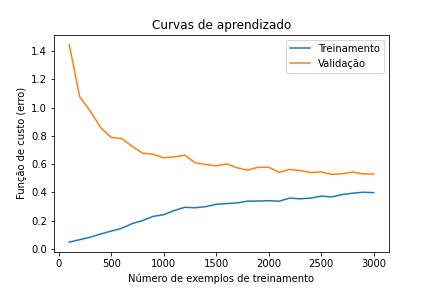
\includegraphics[scale=0.8]{curvas_aprendizado.jpg}
\caption{Curvas de aprendizado.} \label{curvas_aprendizado}\end{center}
\end{figure}

Conforme esperado, o erro do conjunto de treinamento se torna cada vez maior, devido à maior quantidade de exemplos, enquanto para o conjunto de validação o erro diminui, de forma a torná-los cada vez mais próximos. 

\subsection{Seleção de $\lambda$} \label{lambda_otimo}
Nessa Seção, é descrito o procedimento utilizado para encontrar o valor ótimo de $\lambda$ na regularização. Para isso, foram feitos dez treinamentos com o conjunto de treino, todos com 800 iterações e $\alpha=0,8$, variando o valor de $\lambda$ no conjunto $\{0; 0,001; 0,003; 0,01; 0,03; 0,1; 0,3; 1; 3; 10\}$. Para cada treinamento, avaliou-se o erro para o conjunto de validação.

Para analisar o resultado, foram construídos três gráficos:  evolução do erro do conjunto de validação em função de $\lambda$ (Figura \ref{evolucao_lambda}),  evolução do erro do conjunto de validação com relação ao $\lambda$ para os primeiros 6 treinamentos (Figura \ref{primeiros_lambda}) e logaritmo do erro em função do logaritmo de $\lambda$ (Figura \ref{log_lambda}). Os três gráficos são úteis para visualizar o resultado, pois, devido à grande variação de $\lambda$, apenas um deles é insuficiente para perceber os resultados adequadamente.

\begin{figure}
\begin{center}
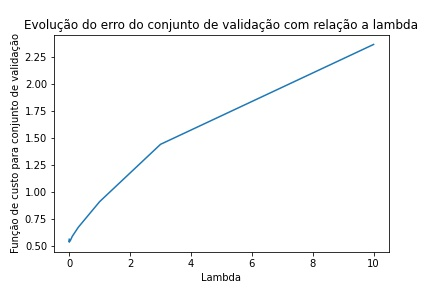
\includegraphics[scale=0.8]{evolucao_lambda.jpg}
\caption{Evolução da função de custo para o conjunto de validação em função de $\lambda$.} \label{evolucao_lambda}
\end{center}
\end{figure}

\begin{figure}
\begin{center}
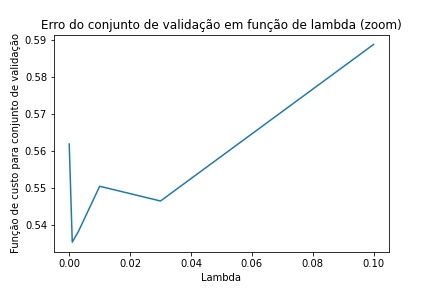
\includegraphics[scale=0.8]{primeiros_lambda.jpg}
\caption{Evolução da função de custo para o conjunto de validação em função dos seis primeiros valores de $\lambda$.} \label{primeiros_lambda}
\end{center}
\end{figure}

\begin{figure}
\begin{center}
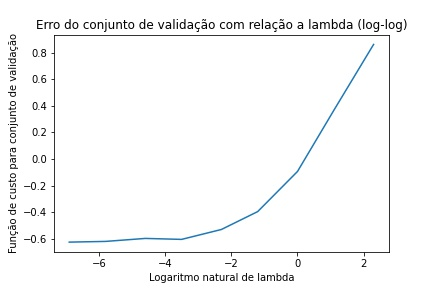
\includegraphics[scale=0.8]{log_lambda.jpg}
\caption{Evolução do logaritmo da função de custo para o conjunto de validação em função do logaritmo de $\lambda$.} \label{log_lambda}
\end{center}
\end{figure}

A partir dos resultados desses treinamentos e da comparação com o desempenho do conjunto de validação, obteve-se 0,001 como valor ótimo para $\lambda$. Com base nesse resultado, novo treinamento foi realizado, dessa vez usando tanto o conjunto de treino quanto o de validação como exemplos, utilizando 800 iterações, $\alpha=0,8$ e $\lambda=0,001$. Avaliou-se, então, o desempenho do método ao aplicá-lo ao conjunto de teste, obtendo classificação correta para 91,6\% das imagens e função de custo avaliada em 0,5319.


\section{Referências}
Vídeo-aulas e \textit{slides} pelo Professor João Batista Florindo em ocasião de oferecimento da disciplina MS960 no segundo semestre de 2020 pelo Instituto de Matemática, Estatística e Computação Científica (IMECC) da Universidade Estadual de Campinas (UNICAMP). Artigo sobre checagem do gradiente presente no seguinte endereço:

https://towardsdatascience.com/how-to-debug-a-neural-network-with-gradient-checking-41deec0357a9

Documentação da função minimize presente no seguinte endereço:

https://docs.scipy.org/doc/scipy/reference/generated/scipy.optimize.minimize.html


\end{document}